% ****************************************************************************************************
\chapter{Simulating the Adoption Process of Platform as a Service Business Models}\label{ch:sfd}
% ****************************************************************************************************

Based on the above discussed qualitative model, within this chapter a quantitative model is developed in order to simulate the adoption process of \ac{PaaS} business models. As with the qualitative model, also for the hereafter introduced quantitative model the concept of system dynamics according to \citet{Sterman2000,Sterman2001} is used. To be more specific, the overall qualitative model respectively \ac{CLD} (cf. Figure \ref{fig:cld_bp}) will be transferred into a quantitative model -- also known as \acf{SFD}. Hereby the third sub-research question will be answered, but also the main research question regarding high-leverage interventions and policies so as to achieve a high adoption rate.

% ****************************************************************************************************
\section{Stocks and Flows}\label{ch:sfd:sf}
% ****************************************************************************************************

The two central concepts of the system dynamics theory are stocks and flows as well as the feedback structure both of the system under investigation. Basically stocks accumulate flows over time. Moreover \textit{"they characterize the state of the system and generate the information upon which decisions and actions are based. Stocks give systems inertia and provide them with memory. Stocks create delays by accumulating the difference between the inflow to a process and its outflow. By decoupling rates of flow, stocks are the source of disequilibrium dynamics in system"} \citep[p. 192]{Sterman2000}.

\begin{figure}[tb]
	\centering
	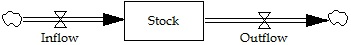
\includegraphics[width=0.5\textwidth]{gfx/sfd_basic}
	\caption[Stock and Flow Diagram -- Basics]{Stock and Flow Diagram -- Basics adapted from \citet[p. 194]{Sterman2000}}
	\label{fig:sfd_b}
\end{figure}

In Figure \ref{fig:sfd_b} the general structure of stocks and flows is illustrated. A stock increases through one or more inflows. These flows can either come from outside the model, thus representing a model boundary (denoted as cloud) or from another stock, hence this kind of flow is an in- and outflow simultaneous (an outflow for stock A and an inflow for stock B). Through one or more outflows stocks decrease over time. These outflows can either represent a model boundary (denoted as cloud) or flow into another stock.

The size of a stock at any time is the accumulation of all its inflows less all its outflows. By using mathematical notation this states as follows: stocks integrate their flows. This leads to the following integral equation in line with \citet[p. 194]{Sterman2000} as shown in  Formula \ref{eq:int}:

\begin{equation}\label{eq:int}
		Stock(t) = \int\limits_{t_0}^t [Inflow(s) - Outflow(s)]ds + Stock(t_0)
\end{equation}

Whereas the $Inflow(s)$ respectively $Outflow(s)$ represent the flow at any time $s$ between the initial time $t_0$ and the current time $t$, and the initial size of the stock is denoted by $Stock(t_0)$. 

Another size of interest is the net rate of change of any stock, its derivative, which is defined by the following differential equation in line with \citet[p. 194]{Sterman2000} as shown in Formula \ref{eq:dif}:

\begin{equation}\label{eq:dif}
		\frac{d(Stock)}{dt} = \mathit{Net~Change~in~Stock} = Inflow(t) - Outflow(t)
\end{equation}

Whereas the $Inflow(t)$ respectively $Ouflow(t)$ represent the flow at the current time $t$.

By applying the above described concept of stocks and flows onto the previous developed \ac{CLD}, 11 crucial stocks in the domain of \ac{PaaS} business models were revealed (cf. Figure \ref{fig:sfd_cs}). The number of all stakeholders using the platform is denoted as customer base and increases through the inflow new customer. However, within this study the time horizon of investigating the platform adoption is rather considered in a short-time horizon. Due to this assumption, the stock customer base does not decrease through a corresponding outflow and simplifies the \ac{SFD} thereby. The remaining ten stocks are dedicated to the five earlier defined customer segments. Each customer segment is modeled as a stock of potential customers (denoted as potential <customer segment>\footnote{The wildcard \texttt{<customer segment>} represents the five earlier identified customer segments.}) and as a second stock of the customer population (denoted as <customer segment> population). These two stocks are linked through the flow adoption rate <customer segment>, whereas this flow decreases the stock potential <customer segment> and increases the stock <customer segment> population. As with the stock customer base, also for the 10 stocks dedicated to the five customer segments corresponding model boundaries have been defined. The <customer segment> population stock does not decrease through an outflow due to the rather short-time horizon -- comparable with the stock customer base. All five potential <customer segment> stocks are defined -- in regards to the initial size -- beforehand the platform adoption simulation is started and decrease over time through the corresponding outflows. These stocks can be defined in two different ways. First, by analyzing the market opportunities of the platform under investigation the numbers of potential customers for the five customer segments can be estimated and used for the simulation. In this case, the simulation will produce absolute values. And second, the simulation can be run using relative values ($0\%$ - $100\%$). In contrast to the first case, here simulation result indicates that at any time $t$ $i\%$ of the customer segment are using the platform (this holds obvious for all customer segments).

\begin{figure}[tb]
	\centering
	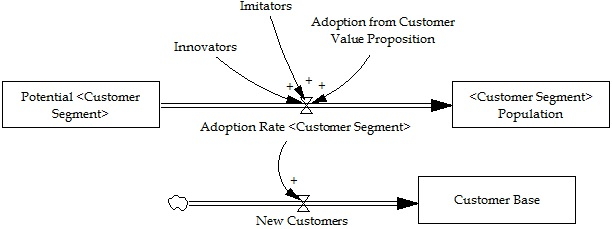
\includegraphics[width=0.8\textwidth]{gfx/sfd_customerSegment}
	\caption{Stock and Flow Diagram -- Generic PaaS Customer Segment}
	\label{fig:sfd_cs}
\end{figure}

The two above described flows -- new customer and adoption rate <customer segment>  -- are influenced as follows. Literally, the inflow new customer is the accumulation of all five customer segment inflows (cf. Formula \ref{eq:nc}). Whereas the adoption rate <customer segment> is the sum of the innovators (cf. Formula \ref{eq:cs:in}), imitators (cf. Formula \ref{eq:cs:im}), as well as through the adoption from the customer value proposition (cf. Formula \ref{eq:cs:acvp}). As already mentioned by \citet[p. 20]{Sterman2001}, his elementary adoption cycle (cf. Figure \ref{fig:cld_ac}) needs to be adapted to circumstances. Thus, in the quantification process the adoption rate has been modeled with the three above mentioned influencing factors. By using these variables the diffusion of innovations theory introduced by \citet{Rogers2003} is taken into account. Thereby the group of innovators, but also early adopters, is considered in the \ac{PaaS} adoption simulation.

Imitators and the adoption from the customer value proposition are mainly influenced by network effects. Imitators are among under things convinced through existing customers within the same customer segment, thus representing a same-sided network effect (cf. the feedback loops R\_1 and B\_1 within Figure \ref{fig:cld_cs}). In contrast to imitators, 'convinced' adopters (adoption from customer value proposition) are starting to use the platform due to the conclusive value proposition which is partly influenced through other customer segments, thus representing cross-sided network effects (cf. the feedback loops identified in Figure \ref{fig:cld_csi}). In Figure \ref{fig:sfd_cs} the above described generic stock and flow structure for the \ac{PaaS} domain is illustrated.

% ****************************************************************************************************
\section{Model Foundations}\label{ch:sfd:mf}
% ****************************************************************************************************
In the following the model foundations are introduced which are necessary so as to simulate the platform adoption. Due to the fact that within the subsequent pages quite a few acronyms are used they are briefly listed in Table \ref{tab:acro} for reasons of clarity and comprehensibility.

\begin{table}[t]
	\centering
	\begin{tabular}{ll}
			\toprule 
			\footnotesize \textbf{Acronym} & \footnotesize \textbf{Meaning}	 \\ \midrule
			\footnotesize \acs{ITS} & \footnotesize \acl{ITS}\\
			\footnotesize \acs{SI} & \footnotesize \acl{SI}\\
			\footnotesize \acs{ISV} & \footnotesize \acl{ISV}\\
			\footnotesize \acs{PC} & \footnotesize \acl{PC}\\
			\footnotesize \acs{AC} & \footnotesize \acl{AC}\\ 
			\footnotesize \acs{CS} & \footnotesize \acl{CS}\\ \midrule
			\footnotesize \acs{GOV} & \footnotesize \acl{GOV}\\
			\footnotesize \acs{TS} & \footnotesize \acl{TS}\\
			\footnotesize \acs{AS} & \footnotesize \acl{AS}\\ \midrule
			\footnotesize \acs{PI} & \footnotesize \acl{PI}\\
			\footnotesize \acs{PM} & \footnotesize \acl{PM}\\
			\footnotesize \acs{MP} & \footnotesize \acl{MP}\\ \midrule
			\footnotesize \acs{CVP} & \footnotesize \acl{CVP}\\
			\footnotesize \acs{AR} & \footnotesize \acl{AR} \\ 
			\footnotesize \acs{IN} & \footnotesize \acl{IN} \\ 
			\footnotesize \acs{IM} & \footnotesize \acl{IM} \\ 
			\footnotesize \acs{ACVP} & \footnotesize \acl{ACVP} \\ 
			\footnotesize \acs{UB} & \footnotesize \acl{UB} \\
			\footnotesize \acs{LB} & \footnotesize \acl{LB}\\
			\footnotesize \acs{P} & \footnotesize \acl{P}\\ \bottomrule
	\end{tabular}
	\caption{Simulation Model Acronyms}
	\label{tab:acro}
\end{table}

As mentioned above, the flow $New~Customer(t)$ is the accumulation of the five customer segment inflows $AR_{CS}(t)$ at any time $t$:

\begin{equation}\label{eq:nc}
	\mathit{New~Customer(t)} = \sum AR_{CS}(t)
\end{equation}

The corresponding stock $Customer~Base(t)$ is simply the initial stock size $\mathit{Customer~Base(t_0)}$ increased by the inflow $New~Customer(s)$:

\begin{equation}\label{eq:cb}
	\mathit{Customer~Base(t)} = \int\limits_{t_0}^t \mathit{[New~Customers(s)]ds} + \mathit{Customer~Base(t_0)}
\end{equation}

By using the stock $Customer~Base(t)$, the overall market penetration $MP_{Overall}(t)$ can be calculated. Due to the model simplifications, this value is the ratio of the $Customer~Base(t)$ to the sum of all current \linebreak ($Customer~Base(t)$) as well as potential ($Potential~CS(t)$) customers:

\begin{equation}\label{eq:mpo}
	MP_{Overall}(t) = \frac{\mathit{Customer~Base(t)}}{\mathit{Customer~Base(t)} + \sum \mathit{Potential~CS(t)}} \in [0.0,1.0]
\end{equation}

Within Section \ref{ch:sfd:mv} and \ref{ch:sfd:mp} the model variables as well as parameters which are used in this simulation model are introduced. These and other values need to be mapped to certain intervals so as to adjust the model dynamics. In order to map the values of the function $f(s) \in [a_1,a_2]$ to the desired interval $[b_1,b_2]$, the following generic linear transformation function is used:

\begin{equation}\label{eq:lt}
	f(l) = b_{1} + \frac{(s-a_1)(b_2-b_1)}{(a_2-a_1)} \in [b_1,b_2]
\end{equation}

In the particaular case of mapping the function $f(s) \in [0,1]$ to the interval $[b_1,b_2]$, the Formula \ref{eq:lt} can be simplified as follows:

\begin{equation}\label{eq:lts}
	f(l) = b_{1} + s (b_{2}-b_{1}) \in [b_{1},b_{2}].
\end{equation}

For the following five formulas this two linear transformation functions -- as appropriate simplified -- are used in order to map the corresponding functions to the desired intervals.

During the investigation of \ac{PaaS} business models, the difference between the pursued governance model have been noticed and considered in the classification scheme as well as \ac{CLD}. In the quantitative model the value of the governance is considered unalterable due to the short-time horizon as well as to the assumption that \ac{PaaS} providers' will not change their governance model from scratch. Therefore the initial governance model value $GOV(t_0)$ is just mapped into the corresponding interval -- between the lower $LB_{GOV}$ and upper boundary $UP_{GOV}$ -- by applying the simplified transformation function as shown in Formula \ref{eq:lts}:

\begin{equation}\label{eq:gov}
	GOV(t) = LB_{GOV} + GOV(t_0) * (UB_{GOV} - LB_{GOV}) \in [LB_{GOV},UB_{GOV}]
\end{equation}

Within the overall \ac{CLD} it was reasoned that an increase in the customer base will increase the revenue above what it would otherwise have been. Furthermore, through the increased revenue the platform investments will increase subsequent and finally resulting in increased platform improvements. However, in the \ac{SFD} this set of facts is simplified for reasons of clarity and comprehensibility. In order to take the quantitative model understandable although its complexity and to avoid adding too many external variables -- assumptions -- to this model, for the variable  platform improvements $PI(t)$ the value of the variable $MP_{Overall}$ (cf. Formula \ref{eq:mpo}) is simply mapped to the desired platform improvements interval by applying Formula \ref{eq:lts}. Behind this simplification -- which is basically in line with \citet[p. 200]{Evans2003} -- was the idea that an increased customer base will finally lead to higher platform improvements:

\begin{equation}\label{eq:pi}
	PI(t) = LB_{PI} + MP_{Overall}(t) * (UB_{PI} - LB_{PI}) \in [LB_{PI},UB_{PI}]
\end{equation}

The next two general values -- technical scope as well as additional services -- are further influencing factors which have been revealed and modeled previously. In contrast to the governance model, for this two factors it is considered that they improve over time through the variable platform improvements $PI(t)$ as calculated in Formula \ref{eq:pi}. Hence, for any time $t$ the actually value for both is calculated by using the initial value $TS(t_0)$ respectively $ AS(t_0)$ and multiplying with the current platform improvements $PI(t)$. This intermediate value is then mapped to the desired interval by applying Formula \ref{eq:lt}. Due to specific intervals for these two variables, the denominator of the Formulas \ref{eq:ts} and \ref{eq:as} is equal to the upper boundary of the platform improvements $UB_{PI}$\footnote{Values for $TS(t_0)$ respectively $AS(t_0)$ are within the interval $[0.0,1.0]$ and for $PI(t)$ within the interval $[1.0,2.0]$ (cf. Section \ref{ch:sfd:mv} and \ref{ch:sfd:mp}). Thus, the intermediate results ($TS(t_0)*PI(t)$ respectively $AS(t_0) *PI(t)$) are within the interval $[0.0,2.0]$ which represents the interval $[a_1,a_2]$ from Formula \ref{eq:lt}. Consequently the denominator for this linear transformation function is $2.0$ ($a_2 - a_1 = 2.0 - 0.0 = 2.0$), equals to $UB_{PI}$. This holds as long as $LB_{TS}$ respectively $LB_{AS}$ is equals to $0.0$.}:

\begin{equation}\label{eq:ts}
	TS(t) = LB_{TS} +  \frac{(TS(t_0) * PI(t)) * (UB_{TS} - LB_{TS})}{UB_{PI}} \in [LB_{TS},UB_{TS}]
\end{equation}

\begin{equation}\label{eq:as}
	AS(t) = LB_{AS} +  \frac{(AS(t_0) * PI(t)) * (UB_{AS} - LB_{AS})}{UB_{PI}} \in [LB_{AS},UB_{AS}]
\end{equation} 

Finally, the variable platform modules -- applications, services, components, or add-ons -- represents the last model foundation. As written above, platform modules are developed and deployed by complementors -- \acp{ISV} and \ac{IT} Startups -- and thus the values of the market penetration of these two customer segments ($MP_{ISV}(t)$ cf. Formula \ref{eq:mp:isv} respectively $MP_{ITS}(t)$ cf. Formula \ref{eq:mp:its}) are used in order to calculate the value of the variable platform modules. This approach was chosen again so as to avoid too many additional assumptions -- parameters, variables, and the like. Therefore the two market penetration values are simply added and mapped to the desired interval by using the linear transformation Formula \ref{eq:lt}. In this particular case, the denominator of the Formula \ref{eq:pm} is equals to the sum of $UB_{ISV}$ and $UB_{ITS}$\footnote{Values for $MP_{ISV}(t)$ respectively $MP_{ITS}(t)$ are within the interval [0.0,1.0] (cf. Section \ref{ch:sfd:mp}). Thus, the addition of $MP_{ISV}(t) + MP_{ITS}(t)$ results in the interval $[0.0,2.0]$ which represents the interval $[a_1,a_2]$ from Formula \ref{eq:lt}. Consequently the denominator for this linear transformation is $2.0$ ($a_2 - a_1 = 2.0 - 0.0 = 2.0$), equals to $UB_{ISV} + UB_{ITS}$.}:

\begin{eqnarray}\label{eq:pm}
	PM(t) = LB_{PM} + \frac{(MP_{ISV}(t) + MP_{ITS}(t)) * (UB_{PM} - LB_{PM})}{UB_{ISV} + UB_{ITS}} \nonumber \\ \in [LB_{PM},UB_{PM}]
\end{eqnarray}

% ****************************************************************************************************
\section{Customer-Specific Formulas}\label{ch:sfd:csf}
% ****************************************************************************************************

In the following the customer-specific formulas are discussed. Based on the two previously developed \acp{CLD} -- generic \ac{PaaS} customer segment (cf. Figure \ref{fig:cld_cs}) and \ac{PaaS} customer segment interdependencies (cf. Figure \ref{fig:cld_csi}) -- hereafter the dedicated \acp{CVP} for all five customer segments are revealed.

As indicated in Figure \ref{fig:cld_cs} the \ac{CVP} for each customer segment is influenced by six variables. The four variables governance model (cf. Formula \ref{eq:gov}), technical scope (cf. Formula \ref{eq:ts}), additional services (cf. Formula \ref{eq:as}), as well as platform improvements (cf. Formula \ref{eq:pi}) are common influencing factors and thus are included in all five corresponding \ac{CVP} functions (cf. Formulas \ref{eq:cvp:isv} - \ref{eq:cvp:pc}). Moreover, the \acp{CVP} are further influenced by the certain customer segments (cf. Figure \ref{fig:cld_csi}), however these influencing factors differs for each customer segment as explained further below. And finally, the core value proposition -- distribution channel, application-based integration, development, and integration -- influences the \acp{CVP} as noted during the 23 explorative case studies. Due to missing data and for reason of intelligibility the core value proposition is in this first version of the quantitative model omitted. Adding this factor to the simulation model would be accompanied by at least 20 external variables\footnote{The impact of the four different core value propositions need to be modeled for all five customer segments, resulting in $4*5=20$ additional external model variables.} and thereby rising the model complexity dramatically.

The \ac{CVP} for complementors -- \acp{ISV} and \ac{IT} startups -- is composed of the four general variables $GOV(t)$, $TS(t)$, $AS(t)$, and $PI(t)$, the initial \ac{CVP} -- $CVP_{ISV}(t_0)$ respectively $ CVP_{ITS}(t_0)$ -- as well as through the market penetration of the application ($MP_{AC}(t)$) and platform customers ($MP_{PC}(t)$):

\begin{eqnarray}\label{eq:cvp:isv}
		CVP_{ISV}(t) & = & CVP_{ISV}(t_0) * GOV(t) * TS(t) * AS(t) * \nonumber \\ & & PI(t) * MP_{AC}(t) * MP_{PC}(t)
\end{eqnarray}

\begin{eqnarray}\label{eq:cvp:its}
		CVP_{ITS}(t) & = & CVP_{ITS}(t_0) * GOV(t) * TS(t) * AS(t) * \nonumber \\ & & PI(t) * MP_{AC}(t) * MP_{PC}(t)
\end{eqnarray}

As with the two previous discussed customer segments, also the \ac{SI} \ac{CVP} is influenced by the four general variables $GOV(t)$, $TS(t)$, $AS(t)$, and $PI(t)$ as well as through the initial \ac{CVP} ($CVP_{SI}(t_0)$). Due to the fact, that \acp{SI} offer consultancy services especially for the two customer segments application as well as platform customers, the \ac{SI} \ac{CVP} is influenced through this two corresponding market penetration values -- $MP_{AC}(t)$ and $MP_{PC}(t)$. Moreover, also the number of platform modules ($PM(t)$) is an indicator for flourishing platform and therefore influences the \ac{SI} \ac{CVP}:

\begin{eqnarray}\label{eq:cvp:si}
		CVP_{SI}(t) & = & CVP_{SI}(t_0) * GOV(t) * TS(t) * AS(t) * \nonumber \\ & & PI(t) * PM(t) * MP_{AC}(t) * MP_{PC}(t)
\end{eqnarray}

The remaining two customer segments -- application and platform customers -- are also influenced by the four general variables $GOV(t)$, $TS(t)$, $AS(t)$, and $PI(t)$ as well as through the initial \ac{CVP} ($CVP_{SI}(t_0)$). In alignment with the \ac{CVP} for \acp{SI}, the number of \acp{SI} offering consultancy services for a certain platform ($MP_{SI}(t)$) positively effects both corresponding \acp{CVP} -- $CVP_{AC}(t)$ as well as $CVP_{PC}(t)$. Moreover and quite important for these two customer segments is the number of available platform modules ($PM(t)$) and thus this figure influences these \acp{CVP} accordingly:

\begin{eqnarray}\label{eq:cvp:ac}
		CVP_{AC}(t) & = & CVP_{AC}(t_0) * GOV(t) * TS(t) * AS(t) * \nonumber \\ & & PI(t) * PM(t) * MP_{SI}(t)
\end{eqnarray}

\begin{eqnarray}\label{eq:cvp:pc}
		CVP_ {PC}(t) & = & CVP_{PC}(t_0) * GOV(t) * TS(t) * AS(t) * \nonumber \\ & & PI(t) * PM(t) * MP_{SI}(t)
\end{eqnarray}

Hereafter the residual customer-specific formulas are introduced. Due to fact that this functions are consistent for all five customer segments the generic notation $CS$ is used in the following and denotes the generic character of this functions. However, within Appendix \ref{ch:app04} all simulation functions are summarized including the specific functions for all five customer segments (cf. Appendix \ref{ch:app04:csf}).

As written above, each customer segment is modeled with two stocks -- potential <customer segment> and <customer segment> population. First, the initial size ($\mathit{Potential~CS(t_0)}$) of the potential customer stock \linebreak ($\mathit{Potential~CS(t)}$) decreases through the corresponding adoption rate \linebreak ($AR_{CS}(t)$, cf. Formula \ref{eq:cs:ar}):

\begin{equation}\label{eq:cs:pot}
	\mathit{Potential~CS(t)} =\mathit{Potential~CS(t_0)} - \int\limits_{t_0}^t  [AR_{CS}(s)]ds
\end{equation}

Whereas the corresponding population stock ($\mathit{Population~CS(t)}$) \linebreak increases, on top of the initial stock size ($\mathit{Population~CS(t_0)}$), through the corresponding adoption rate ($AR_{CS}(t)$, cf. Formula \ref{eq:cs:ar}):

\begin{equation}\label{eq:cs:pop}
	\mathit{Population~CS(t)} = \int\limits_{t_0}^t [AR_{CS}(s)]ds + \mathit{Population~CS(t_0)}
\end{equation}

Within this work, three different adopter groups have been identified. Thus the adoption rate ($AR_{CS}(t)$) is the sum of the variables innovators ($IN_{CS}(t)$, cf. Formula \ref{eq:cs:in}), imitators ($IM_{CS}(t)$, cf. Formula \ref{eq:cs:im}), and adoption from the customer value proposition ($ACVP_{CS}(t)$, cf. Formula \ref{eq:cs:acvp}):

\begin{equation}\label{eq:cs:ar}
		AR_{CS}(t) = IN_{CS}(t) + IM_{CS}(t) + ACVP_{CS}(t)	
\end{equation}

The ratio how many customers of a specific customer segment are using the platform, is required for a few calculations below. For this purpose, the current customers ($\mathit{Population~CS(t)}$) are divided by the overall size of customer segment ($\mathit{Population~CS(t)} + \mathit{Potential~CS(t)})$:

\begin{equation}\label{eq:cs:ratio}
		RATIO_{CS}(t) = \frac{\mathit{Population~CS(t)}}{\mathit{Population~CS(t)} + \mathit{Potential~CS(t)}} \in [0.0,1.0]
\end{equation}

By using this ratio, which actually represent the plain market penetration within the interval $[0.0,1.0]$, the desired market penetration can be calculated by applying Formula \ref{eq:lts} and mapping $RATIO_{CS}(t)$ into the desired interval:

\begin{eqnarray}\label{eq:cs:mp}
	MP_{CS}(t) = LB_{MP_{CS}} + RATIO_{CS}(t) * (UB_{MP_{CS}} - LB_{MP_{CS}})  \nonumber \\ \in [LB_{MP_{CS}},UB_{MP_{CS}}]
\end{eqnarray}

The remaing three adopter groups are calculated as follows: Innovators are simply determined by the product of the probability of innovators ($P_{IN_{CS}}$) and the corresponding potential customer stock size \linebreak ($\mathit{Potential~CS(t)}$):

\begin{equation}\label{eq:cs:in}
		IN_{CS}(t) = \mathit{Potential~CS(t)} * P_{IN_{CS}}
\end{equation}

In order to calculate the variable imitators, the probability of imitators ($P_{IM_{CS}}$) is multiplied with the corresponding customer segment ratio ($RATIO_{CS}(t)$). This intermediate result is then further multiplied with the potential customer stock size ($\mathit{Potential~CS(t)}$). By including the variavle $RATIO_{CS}(t)$ into the imitator calculation, this function results in the desired s-shaped curve. Basically, the variable $RATIO_{CS}(t)$ increases and the variable $\mathit{Potential~CS(t)}$ decreases all the time and thus providing the s-shaped curve:

\begin{equation}\label{eq:cs:im}
		IM_{CS}(t) = \mathit{Potential~CS(t)} * P_{IM_{CS}} * RATIO_{CS}(t)
\end{equation}

And finally the adoption from the customer value proposition \linebreak ($ACVP_{CS}(t)$) is similarly to the imitator function the product of the potential customers ($\mathit{Potential~CS(t)}$), the customer segment ratio ($RATIO_{CS}(t)$), and the corresponding customer segment \ac{CVP} ($CVP_{CS}(t)$, cf. Formulas \ref{eq:cvp:isv} - \ref{eq:cvp:pc}). Also this function results in line with Formula \ref{eq:cs:im} in a s-shaped curve:

\begin{equation}\label{eq:cs:acvp}
		ACVP_{CS}(t) = \mathit{Potential~CS(t)} * CVP_{CS}(t) * RATIO_{CS}(t)
\end{equation}

% ****************************************************************************************************
\section{Model Variables}\label{ch:sfd:mv}
% ****************************************************************************************************

In order to simulate the \ac{PaaS} business model adoption using the above introduced model foundations, 18 model variables need to be defined, before the simulation can be started. These 18 model variables and their corresponding codomains are presented in Table \ref{tab:mvar}. The variables itself haven been derived directly from the simulation model (\ac{SFD}), in combination with the \ac{CLD} whereupon the \ac{SFD} is built upon. In contrast, the corresponding codomains have been defined by analyzing the model characteristics -- especially the mathematical model and its properties -- and how the above defined formulas correlate. This analysis resulted in the here presented intervals and was reviewed with several experts. In the following all variables and their codomains are briefly discussed.

Within the first column in Table \ref{tab:mvar} three important model variables are illustrated. First, the pursued governance model between the \ac{PaaS} platforms differ notable and thus need to be taken into account in the simulation. Whereas in the classification scheme a qualitative ordinal scale was chosen, in the case of the simulation model a quantitative scale is required. Therefore, the governance model variable can attain values within the interval $[0.0,1.0]$, whereby the value $0.0$ stands for a strictly limited and the value $1.0$ for an open governance model. The next two variables -- technical scope and additional services -- are further essential factors in the \ac{PaaS} adoption process. Also these two variables can attain values within the interval $[0.0,1.0]$, whereby the value $0.0$ represent limited technical capabilities respectively few additional services and the value $1.0$ extensive technical capabilities respectively various additional services.

\newlength{\originalTabcolsep}
\setlength{\originalTabcolsep}{\tabcolsep}
\setlength{\tabcolsep}{1.5mm}

\begin{table}[t]
	\centering
	\begin{tabular}{llllllll}
		\toprule 
		\multicolumn{8}{c}{\footnotesize \textbf{Model Variables and their corresponding Codomains}} \\ \midrule
		\footnotesize $GOV(t_0)$ & \footnotesize $[0.0,1.0]$ & \footnotesize $CVP_{ITS}(t_0)$ & \footnotesize $[0.0,0.1]$ & \footnotesize $P_{IN_{ITS}}$ & \footnotesize $(0.0,0.025]$ & \footnotesize $P_{IM_{ITS}}$ & \footnotesize $[0.0,0.05]$ \\
		\footnotesize $TS(t_0)$ & \footnotesize $[0.0,1.0]$ & \footnotesize $CVP_{SI}(t_0)$ & \footnotesize $[0.0,0.1]$ & \footnotesize $P_{IN_{SI}}$ & \footnotesize $(0.0,0.025]$ & \footnotesize $P_{IM_{SI}}$ & \footnotesize $[0.0,0.05]$ \\
		\footnotesize $AS(t_0)$ & \footnotesize $[0.0,1.0]$ & \footnotesize $CVP_{ISV}(t_0)$ & \footnotesize $[0.0,0.1]$ & \footnotesize $P_{IN_{ISV}}$ & \footnotesize $(0.0,0.025]$ & \footnotesize $P_{IM_{ISV}}$ & \footnotesize $[0.0,0.05]$ \\
		& & \footnotesize $CVP_{PC}(t_0)$ & \footnotesize $[0.0,0.1]$ & \footnotesize $P_{IN_{PC}}$ & \footnotesize $(0.0,0.025]$ & \footnotesize $P_{IM_{PC}}$ & \footnotesize $[0.0,0.05]$ \\
		& & \footnotesize $CVP_{AC}(t_0)$ & \footnotesize $[0.0,0.1]$ & \footnotesize $P_{IN_{AC}}$ & \footnotesize $(0.0,0.025]$ & \footnotesize $P_{IM_{AC}}$ & \footnotesize $[0.0,0.05]$ \\ \bottomrule
	\end{tabular}
	\caption{Model Variables}
	\label{tab:mvar}
\end{table}

\setlength{\tabcolsep}{\originalTabcolsep}

As already discussed in Subsection \ref{ch:tf:bmc} and Section \ref{ch:cld:cs}, each customer segment receive their own dedicated \ac{CVP}, as highlighted by \citet{Johnson2008}. Hence, for all five customer segments the initial \ac{CVP} need to be defined. These five model variables are illustrated in column two within Table \ref{tab:mvar}. Based on the model characteristics reasonable values for the initial \acp{CVP} are within the interval $[0.0,0.1]$.

The remaining ten model variables are used to model the adoption diffusion, especially in the beginning of the adoption process. In alignment with \citet[p. 19]{Sterman2001}, the probability of imitators needs to be defined for all five customer segments independently as illustrated in column four in Table \ref{tab:mvar}. These adopters start to use the platform based on same-sided network effects as calculated in Formula \ref{eq:cs:im}. Values for the probability of imitators for all customer segments are typically in the interval $[0.0, 0.05]$. Due to the fact that these values remain constant for the whole simulation, these intervals are rather small and at the bottom of the scale so as to avoid too high and unrealistic adoption rates and by association a too fast adoption of the platform.

Finally, also the probability of innovators need to be defined for all five customer segments, as illustrated in column three in Table \ref{tab:mvar}. For these probabilities an even smaller interval at the bottom of the scale was chosen: $(0.0,0.025]$. This small interval was designed due to the fact, that these adopter group is just calculated by using the corresponding innovator probability and the corresponding potential customers as shown in Formula \ref{eq:cs:in}. Moreover, the Formulas \ref{eq:cs:im} and \ref{eq:cs:acvp} can result in the value $0$, in case the corresponding customer segment ratio (cf. Formula \ref{eq:cs:ratio}) is still zero. In other words, the adoption from these two adopter groups is nonexistent in the above described scenario. Therefore, the values for the probability of innovators need to be always greater than $0.0$, because this adopter group is calculated without the customer segment ratio and results for probabilities greater than $0.0$ in values greater null (representing innovators), as shown in Formula \ref{eq:cs:in}. Basically, the adoption process starts always with this adopter group -- the innovators -- and thus the above described guidelines arise.


% ****************************************************************************************************
\section{Model Parameters}\label{ch:sfd:mp}
% ****************************************************************************************************

\begin{table}[t]
	\centering
	\begin{tabular}{ll}
			\toprule 
			\footnotesize \textbf{Parameter} & \footnotesize \textbf{Interval} \\ \midrule
			\footnotesize PI & \footnotesize $[1.0,2.0] \implies LB_{PI} = 1.0$ and $UB_{PI}$ = 2.0 \\ 
			\footnotesize PM & \footnotesize  $[1.0,2.0] \implies LB_{PM} = 1.0$ and $UB_{PM}$ = 2.0 \\ \midrule
			\footnotesize GOV & \footnotesize $[1.0,1.1] \implies LB_{GOV} = 1.0$ and $UB_{GOV}$ = 1.1 \\
			\footnotesize TS & \footnotesize $[1.0,1.1] \implies LB_{TS} = 1.0$ and $UB_{TS}$ = 1.1 \\
			\footnotesize AS & \footnotesize $[1.0,1.1] \implies LB_{AS} = 1.0$ and $UB_{AS}$ = 1.1 \\ \midrule
			\footnotesize $MP_{ITS}$ & \footnotesize $[0.0,1.0] \implies LB_{ITS} = 0.0$ and $UB_{ITS}$ = 1.0 \\
			\footnotesize $MP_{ISV}$ & \footnotesize $[0.0,1.0] \implies LB_{ISV} = 0.0$ and $UB_{ISV}$ = 1.0 \\
			\footnotesize $MP_{AC}$ & \footnotesize $[1.0,2.0] \implies LB_{AC} = 1.0$ and $UB_{AC}$ = 2.0 \\
			\footnotesize $MP_{SI}$ & \footnotesize $[1.0,1.1] \implies LB_{SI} = 1.0$ and $UB_{SI}$ = 1.1 \\
			\footnotesize $MP_{PC}$ & \footnotesize $[1.0,1.2] \implies LB_{PC} = 1.0$ and $UB_{PC}$ = 1.2 \\ \bottomrule
	\end{tabular}
	\caption{Model Parameters}
	\label{tab:mpara}
\end{table}
